\chapter{Additional Results}
\label{chapter:appendix-results}

This appendix contains additional results of our experiments which complement chapter \ref{chapter:results}.

\begin{figure}[]
    \centering    
    \begin{subfigure}{\textwidth}
        \centering
        \begin{subfigure}{0.24\textwidth}
            \centering
            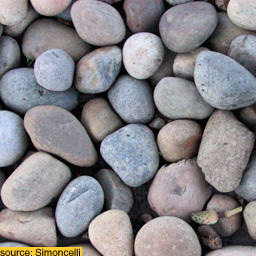
\includegraphics[width=\textwidth]{images/04-experiment01/pebbles/target.jpg}
            \caption*{}
        \end{subfigure}
        \hfill
        \begin{subfigure}{0.24\textwidth}
            \centering
            
\includegraphics[width=\textwidth]{images/04-experiment01/pebbles/white_bg.jpg}
            \caption*{}
        \end{subfigure}
        \hfill
        \begin{subfigure}{0.24\textwidth}
            \centering
            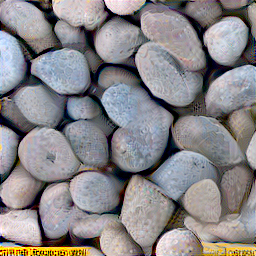
\includegraphics[width=\textwidth]{images/04-experiment01/pebbles/1000/white_im.jpg}
            \caption*{}
        \end{subfigure}
        \hfill
        \begin{subfigure}{0.24\textwidth}
            \centering
            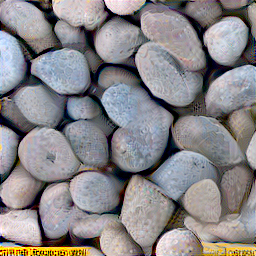
\includegraphics[width=\textwidth]{images/04-experiment01/pebbles/1000/white_proj.jpg}
            \caption*{}
        \end{subfigure}

        \begin{subfigure}{0.24\textwidth}
            \centering
            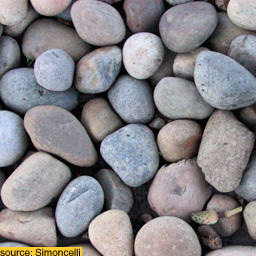
\includegraphics[width=\textwidth]{images/04-experiment01/pebbles/target.jpg}
            \caption*{}
        \end{subfigure}
        \hfill
        \begin{subfigure}{0.24\textwidth}
            \centering
            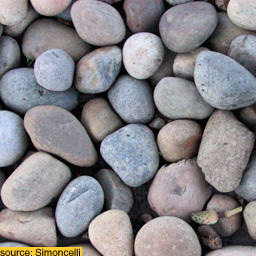
\includegraphics[width=\textwidth]{images/04-experiment01/pebbles/pebbles_bg.jpg}
            \caption*{}
        \end{subfigure}
        \hfill
        \begin{subfigure}{0.24\textwidth}
            \centering
            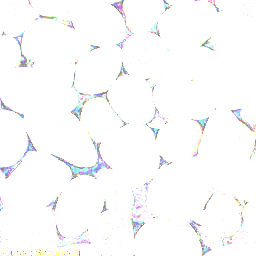
\includegraphics[width=\textwidth]{images/04-experiment01/pebbles/1000/pebbles_im.jpg}
            \caption*{}
        \end{subfigure}
        \hfill
        \begin{subfigure}{0.24\textwidth}
            \centering
            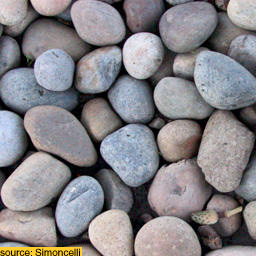
\includegraphics[width=\textwidth]{images/04-experiment01/pebbles/1000/pebbles_proj.jpg}
            \caption*{}
        \end{subfigure}

        \begin{subfigure}{0.24\textwidth}
            \centering
            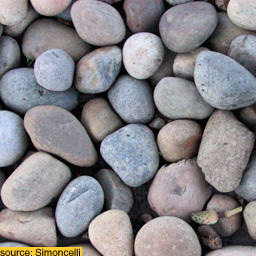
\includegraphics[width=\textwidth]{images/04-experiment01/pebbles/target.jpg}
            \caption*{}
        \end{subfigure}
        \hfill
        \begin{subfigure}{0.24\textwidth}
            \centering
            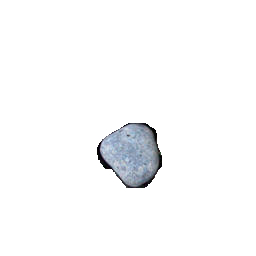
\includegraphics[width=\textwidth]{images/04-experiment01/pebbles/one_bg.jpg}
            \caption*{}
        \end{subfigure}
        \hfill
        \begin{subfigure}{0.24\textwidth}
            \centering
            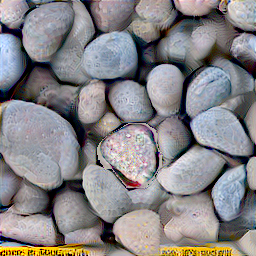
\includegraphics[width=\textwidth]{images/04-experiment01/pebbles/1000/one_im.jpg}
            \caption*{}
        \end{subfigure}
        \hfill
        \begin{subfigure}{0.24\textwidth}
            \centering
            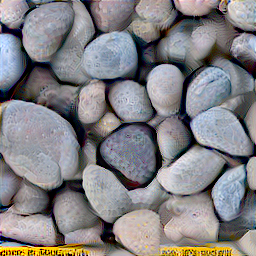
\includegraphics[width=\textwidth]{images/04-experiment01/pebbles/1000/one_proj.jpg}
            \caption*{}
        \end{subfigure}

        \begin{subfigure}{0.24\textwidth}
            \centering
            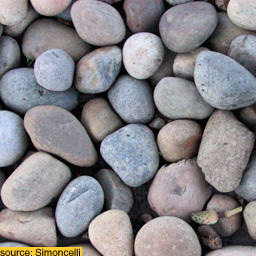
\includegraphics[width=\textwidth]{images/04-experiment01/pebbles/target.jpg}
            \caption*{}
        \end{subfigure}
        \hfill
        \begin{subfigure}{0.24\textwidth}
            \centering
            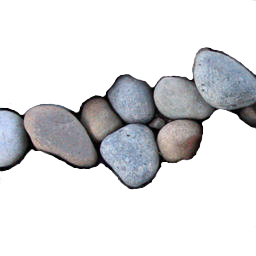
\includegraphics[width=\textwidth]{images/04-experiment01/pebbles/some_bg.jpg}
            \caption*{}
        \end{subfigure}
        \hfill
        \begin{subfigure}{0.24\textwidth}
            \centering
            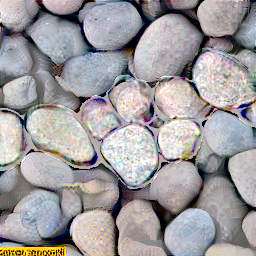
\includegraphics[width=\textwidth]{images/04-experiment01/pebbles/1000/some_im.jpg}
            \caption*{}
        \end{subfigure}
        \hfill
        \begin{subfigure}{0.24\textwidth}
            \centering
            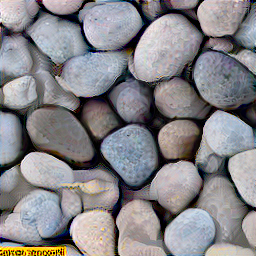
\includegraphics[width=\textwidth]{images/04-experiment01/pebbles/1000/some_proj.jpg}
            \caption*{}
        \end{subfigure}
        
        \begin{subfigure}{0.24\textwidth}
            \centering
            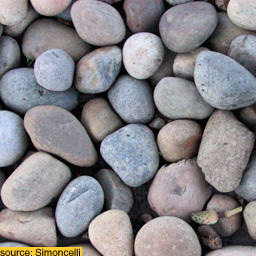
\includegraphics[width=\textwidth]{images/04-experiment01/pebbles/target.jpg}
            \caption*{Input}
        \end{subfigure}
        \hfill
        \begin{subfigure}{0.24\textwidth}
            \centering
            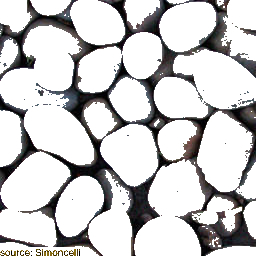
\includegraphics[width=\textwidth]{images/04-experiment01/pebbles/threshold_bg.jpg}
            \caption*{Background}
        \end{subfigure}
        \hfill
        \begin{subfigure}{0.24\textwidth}
            \centering
            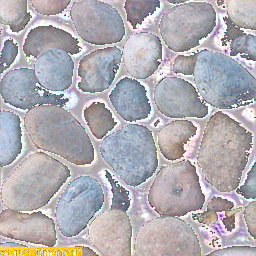
\includegraphics[width=\textwidth]{images/04-experiment01/pebbles/1000/threshold_im.jpg}
            \caption*{Compensation}
        \end{subfigure}
        \hfill
        \begin{subfigure}{0.24\textwidth}
            \centering
            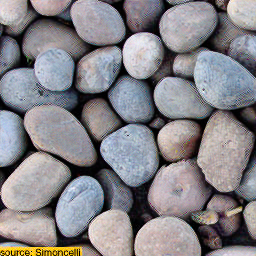
\includegraphics[width=\textwidth]{images/04-experiment01/pebbles/1000/threshold_proj.jpg}
            \caption*{Camera image}
        \end{subfigure}
    \end{subfigure}
    \caption{These results complement section \ref{section:results-experiments-01}. Texture source: \citet{Gatys2015}}
    \label{fig:ex01-complete-pebbles-1000steps}
\end{figure}

\begin{figure}[]
    \centering    
    \begin{subfigure}{\textwidth}
        \centering
        \begin{subfigure}{0.24\textwidth}
            \centering
            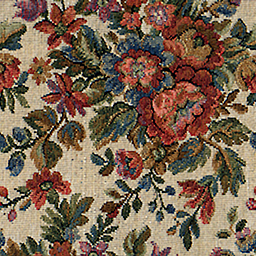
\includegraphics[width=\textwidth]{images/04-experiment01/flowers/target.jpg}
            \caption*{}
        \end{subfigure}
        \hfill
        \begin{subfigure}{0.24\textwidth}
            \centering
            
\includegraphics[width=\textwidth]{images/04-experiment01/flowers/white_bg.jpg}
            \caption*{}
        \end{subfigure}
        \hfill
        \begin{subfigure}{0.24\textwidth}
            \centering
            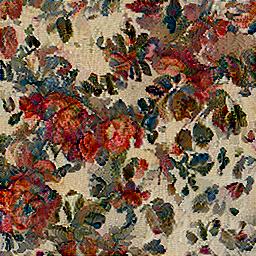
\includegraphics[width=\textwidth]{images/04-experiment01/flowers/1000/white_im.jpg}
            \caption*{}
        \end{subfigure}
        \hfill
        \begin{subfigure}{0.24\textwidth}
            \centering
            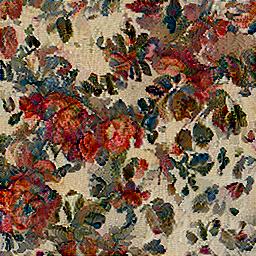
\includegraphics[width=\textwidth]{images/04-experiment01/flowers/1000/white_proj.jpg}
            \caption*{}
        \end{subfigure}

        \begin{subfigure}{0.24\textwidth}
            \centering
            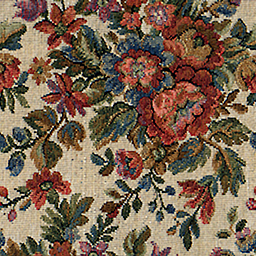
\includegraphics[width=\textwidth]{images/04-experiment01/flowers/target.jpg}
            \caption*{}
        \end{subfigure}
        \hfill
        \begin{subfigure}{0.24\textwidth}
            \centering
            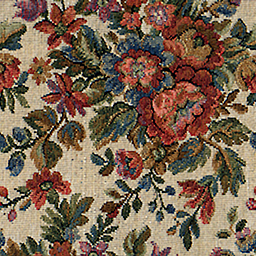
\includegraphics[width=\textwidth]{images/04-experiment01/flowers/flowers_bg.jpg}
            \caption*{}
        \end{subfigure}
        \hfill
        \begin{subfigure}{0.24\textwidth}
            \centering
            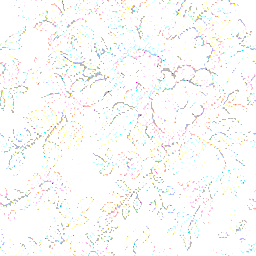
\includegraphics[width=\textwidth]{images/04-experiment01/flowers/1000/flowers_im.jpg}
            \caption*{}
        \end{subfigure}
        \hfill
        \begin{subfigure}{0.24\textwidth}
            \centering
            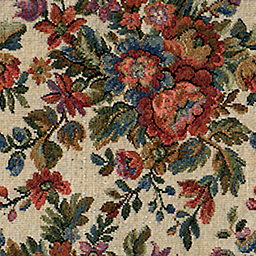
\includegraphics[width=\textwidth]{images/04-experiment01/flowers/1000/flowers_proj.jpg}
            \caption*{}
        \end{subfigure}

        \begin{subfigure}{0.24\textwidth}
            \centering
            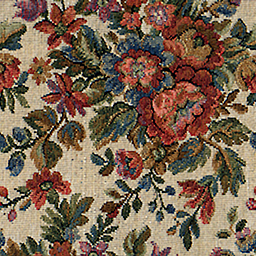
\includegraphics[width=\textwidth]{images/04-experiment01/flowers/target.jpg}
            \caption*{}
        \end{subfigure}
        \hfill
        \begin{subfigure}{0.24\textwidth}
            \centering
            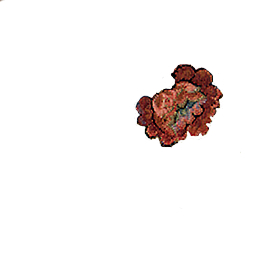
\includegraphics[width=\textwidth]{images/04-experiment01/flowers/one_bg.jpg}
            \caption*{}
        \end{subfigure}
        \hfill
        \begin{subfigure}{0.24\textwidth}
            \centering
            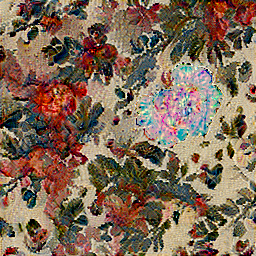
\includegraphics[width=\textwidth]{images/04-experiment01/flowers/1000/one_im.jpg}
            \caption*{}
        \end{subfigure}
        \hfill
        \begin{subfigure}{0.24\textwidth}
            \centering
            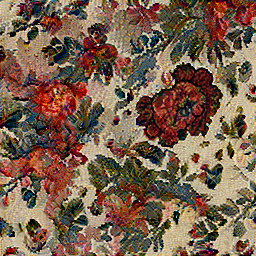
\includegraphics[width=\textwidth]{images/04-experiment01/flowers/1000/one_proj.jpg}
            \caption*{}
        \end{subfigure}

        \begin{subfigure}{0.24\textwidth}
            \centering
            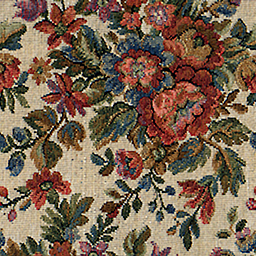
\includegraphics[width=\textwidth]{images/04-experiment01/flowers/target.jpg}
            \caption*{}
        \end{subfigure}
        \hfill
        \begin{subfigure}{0.24\textwidth}
            \centering
            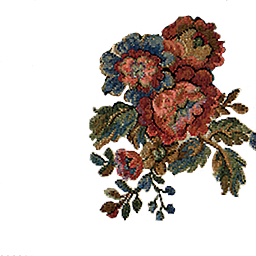
\includegraphics[width=\textwidth]{images/04-experiment01/flowers/some_bg.jpg}
            \caption*{}
        \end{subfigure}
        \hfill
        \begin{subfigure}{0.24\textwidth}
            \centering
            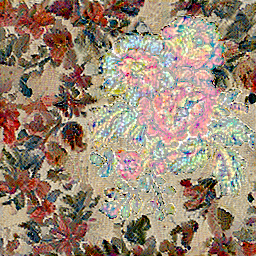
\includegraphics[width=\textwidth]{images/04-experiment01/flowers/1000/some_im.jpg}
            \caption*{}
        \end{subfigure}
        \hfill
        \begin{subfigure}{0.24\textwidth}
            \centering
            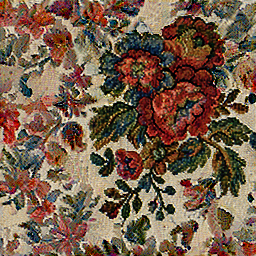
\includegraphics[width=\textwidth]{images/04-experiment01/flowers/1000/some_proj.jpg}
            \caption*{}
        \end{subfigure}
        
        \begin{subfigure}{0.24\textwidth}
            \centering
            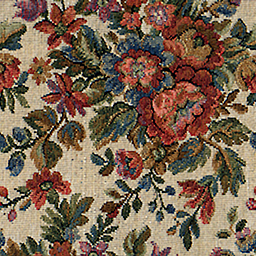
\includegraphics[width=\textwidth]{images/04-experiment01/flowers/target.jpg}
            \caption*{Input}
        \end{subfigure}
        \hfill
        \begin{subfigure}{0.24\textwidth}
            \centering
            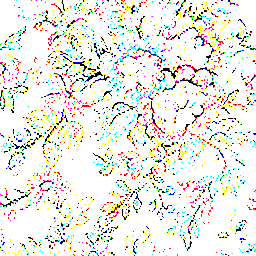
\includegraphics[width=\textwidth]{images/04-experiment01/flowers/threshold_bg.jpg}
            \caption*{Background}
        \end{subfigure}
        \hfill
        \begin{subfigure}{0.24\textwidth}
            \centering
            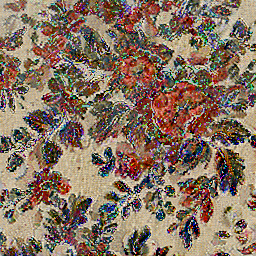
\includegraphics[width=\textwidth]{images/04-experiment01/flowers/1000/threshold_im.jpg}
            \caption*{Compensation}
        \end{subfigure}
        \hfill
        \begin{subfigure}{0.24\textwidth}
            \centering
            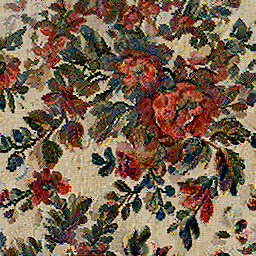
\includegraphics[width=\textwidth]{images/04-experiment01/flowers/1000/threshold_proj.jpg}
            \caption*{Camera image}
        \end{subfigure}
    \end{subfigure}
    \caption{These results complement section \ref{section:results-experiments-01}. Texture source: \citet{Gatys2015}}
    \label{fig:ex01-complete-flowers-1000steps}
\end{figure}

\chapter{Convolutional Neural Networks}
\label{chapter:appendix-cnns}

{\color{red} TODO: in-depth explanation of CNNs here for completeness}

\textit{Neural networks}, or more precisely \textit{feedforward neural networks}, are essentially functions

\begin{equation}
    \label{eq:neural_network}
    y = f(x, \phi)
\end{equation}

where \(x\) is the input, \(y\) is the output and \(\phi\) are the parameters of a neural network. The idea is that \(f\) is an approximation of \(f^\star\) which is a very complex, non-linear function which tells us something about the world. For example, we can consider \(f^\star\) to be the mapping between all possible images of size \(224 \times 224\) and categories such as dog, cat, tree, house, etc. that describe the image. The goal of \textit{deep learning}, which is the study of feedforward and other kinds of neural networks, is then to find an \(f\) along with its parameters \(\phi\) that approximate \(f^\star\) as closely as possible. Because of the complexity of \(f^\star\), \(f(x) = f^{(3)}(f^{(2)}(f^{(1})(x)))\) is often composed of many functions \(f^{(i)}\) which are called \textit{layers}. Each layer usually operates on vectors and is commposed of small units that are loosely modeled on brain neurons. Together, these layers form a network where information flows from the first layer to the last. Hence the term \textit{feedforward neural network}.

{\color{red} TODO: mention training?}

Convolutional neural networks (CNNs) form a class of neural networks that are intended for processing grid-like inputs, for example images (2D grid) or audio (1D grid). Their layers are typically composed of three parts: convolution, nonlinearity and pooling.

{\color{red} TODO: image}

\textbf{Convolution}. To explain convolution in the context of neural networks, it is best to start with an example. Let us imagine that we have an image and would like to find all vertical edges in that image. This can be done using convolution ({\color{red} TODO: image}). All we need to do is take a \(3 \times 3\) matrix ({\color{red} TODO: figure out the right values\dots}), also called \(kernel\), move it across the image aligning the center of the kernel with each image pixel in turn, multiplying overlapping values, summing them together and writing them out into a new image. We will notice that the new image contains high values in places where there is a vertical edge in the original image. What has happened?

The process we have gone through with our image and our kernel is called convolution in the context of deep learning, although strictly speaking, it corresponds to cross-correlation which differs from convolution by the orientation of the kernel. Our kernel happens have values which detect vertical edges when convolved with an image. Kernels with different values do different things, for example detect horizontal edges, blur the image, or even leave it untouched ({\color{red} TODO: examples!}).

Kernel values are what constitutes the parameters \(\phi\) of a CNN and it turns out that they are powerful enough to achieve impressive results in tasks such as object recognition, ({\color{red} TODO: more examples}). They cannot function alone, however. As we have mentioned, neural networks usually approximate complex non-linear function and convolutions as presented here are linear. Two more building blocks are therefore needed.

\textbf{Nonlinearity}. Nonlinearities are scalar functions whose purpose is to simply introduce nonlinear behavior into a CNN. Many types of nonlinearities have been proposed in recent years, for example hyperbolic tangent or ReLU ({\color{red} TODO: figures}). ReLU is used more commonly simply because it improves results ({\color{red} TODO: maybe cite some justification for this?}).

\textbf{Pooling}. Pooling functions are function that accept a vector as input and return a scalar as output. They are often use to make CNNs invariant to small shifts in the input image and also reduce the size of the intermediate outputs, also called \textit{activations}, of each CNN layer. ({\color{red} TODO: a bit more explanation with images?})

CNNs typically have multiple such layers and since they are trained to classify images, the have a few fully connected layers ({\color{red} TODO:  explain?}) at the end which compress the activations into an \(n\)-dimensional vector where each position of the vector corresponds to a particular image class and the value at that position tells how likely the input image is to belong to that image class. For a more comprehensive overview of neural networks and deep learning, see \citet{Goodfellow2016}. We will now focus how CNNs are related to texture synthesis.

{\color{red} TODO: depth of output? number of feature maps? RGB channels?}

{\color{red} TODO: biases?}

{\color{red} TODO: fully connected layers? classification output?}

For texture synthesis as introduced by \citet{Gatys2015}, however, it is only the activations after individual convolution layers that matter. The operation of convolution and the fact that the network is trained to classify images ({\color{red} TODO: deep image prior?}) causes those activations to contain filtered versions of the input image where particular features that define a texture are emphasized ({\color{red} TODO: now it would be great to have a visualization of which features are picked out at which levels!}).

\chapter{Thin Lens Projector Model}
\label{chapter:appendix-projector}

{\color{red} TODO: in-depth explanation of the thin lens projector model here for completeness}
